\testfile{pgfplotstest.misc.tex}
\testsection{Paths after addplot}
\testsubsection{plot coordinates}
\testsubsubsection{without space after 'coordinates'}
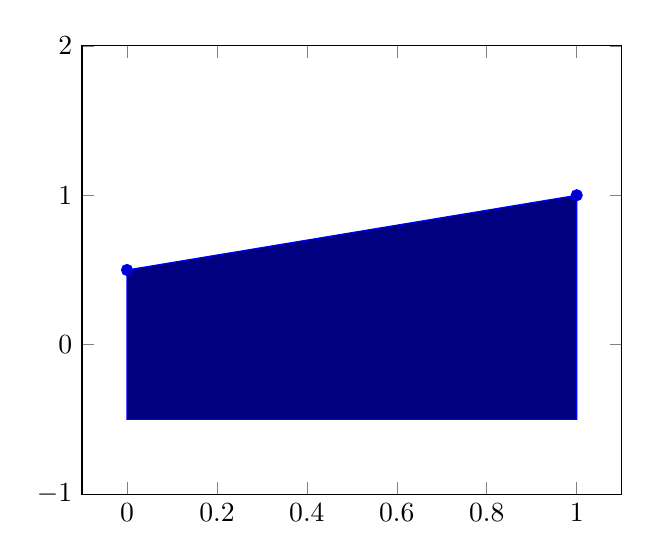
\begin{tikzpicture}
\begin{axis}[ymin=-1,ymax=2]
\addplot+[fill=blue!50!black] coordinates{(0,0.5) (1,1)} |- (axis cs:0,-0.5) -- cycle;
\end{axis}
\end{tikzpicture}

\testsubsubsection{with space after 'coordinates'}
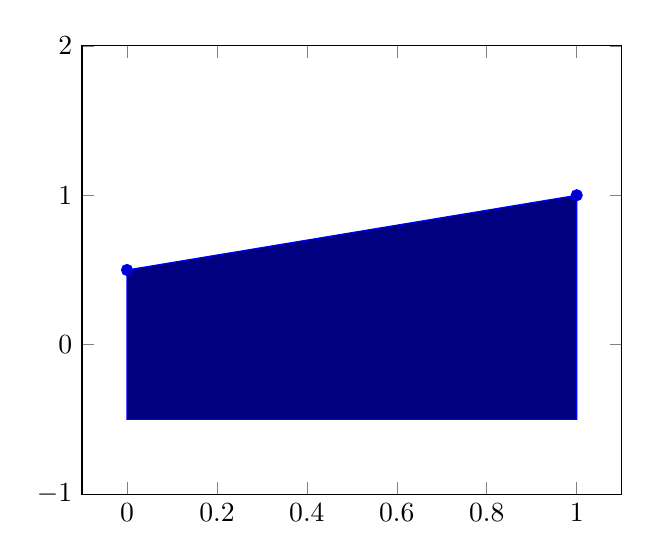
\begin{tikzpicture}
\begin{axis}[ymin=-1,ymax=2]
\addplot+[fill=blue!50!black] coordinates {(0,0.5) (1,1)} |- (axis cs:0,-0.5) -- cycle;
\end{axis}
\end{tikzpicture}

\testsubsubsection{using closedcycle path}
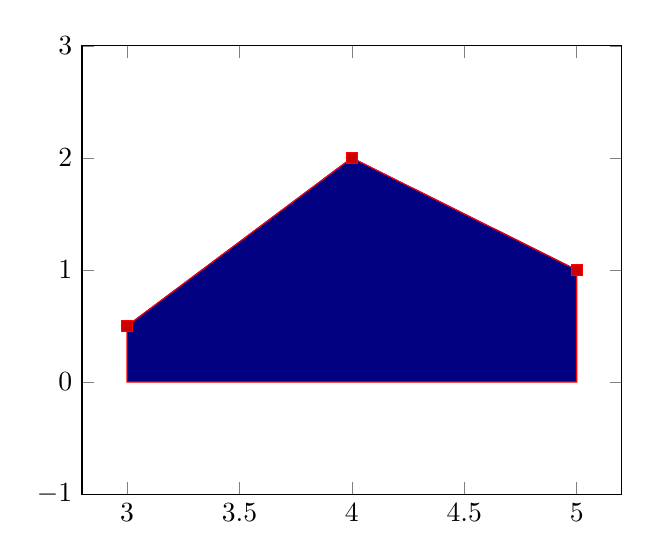
\begin{tikzpicture}
\begin{axis}[ymin=-1,ymax=3]
\addplot coordinates {(3,0.5) (4,2) (5,1)} ;
\addplot+[fill=blue!50!black] coordinates {(3,0.5) (4,2) (5,1)} 
	\closedcycle;
\end{axis}
\end{tikzpicture}

\testsubsection{plot table}
\begin{tikzpicture}
\begin{axis}
\addplot+[fill=blue!50!black] table[x index=0,y index=1,header=false]{plotdata/pgfplotstest_plot2.gnuplot} |- (axis cs:0,-1) -- cycle;
\end{axis}
\end{tikzpicture}

\testsubsection{plot function}
\begin{tikzpicture}
\begin{axis}
\addplot plot[id=parable,domain=-5:5] function{4*x**2 - 5} node[pin=180:{$4x^2-5$}]{};
\end{axis}
\end{tikzpicture}


\testsection{Title-option}
\begin{tikzpicture}
\begin{loglogaxis}[title=A test title,xlabel=Dof,ylabel=Error]
\loglogtestplot
\end{loglogaxis}
\end{tikzpicture}

\testsection{Filter test}
{%
\def\myOwnYfilter#1\to#2{%
	\def#2{0.5}%
}%
\begin{tikzpicture}
%
\begin{axis}[yfilter={\myOwnYfilter}]
\addplot plot coordinates {
	(4,0)
	(6,1)
};
\end{axis}
\end{tikzpicture}

\begin{tikzpicture}
\begin{axis}[y filter/.code={\def\pgfmathresult{0.5}}]
\addplot plot coordinates {
	(4,0)
	(6,1)
};
\end{axis}
\end{tikzpicture}

\begin{tikzpicture}
\begin{axis}[x filter/.code={\ifnum\coordindex>4\def\pgfmathresult{}\fi}]
\addplot (\x,\x^2);
\end{axis}
\end{tikzpicture}
}%

\testsection{Test for addplot+[...]}
{
\pgfplotsset{every axis legend/.append style={at={(1.03,1)},anchor=north west}}
\begin{enumerate}
	\item Ohne aenderung:

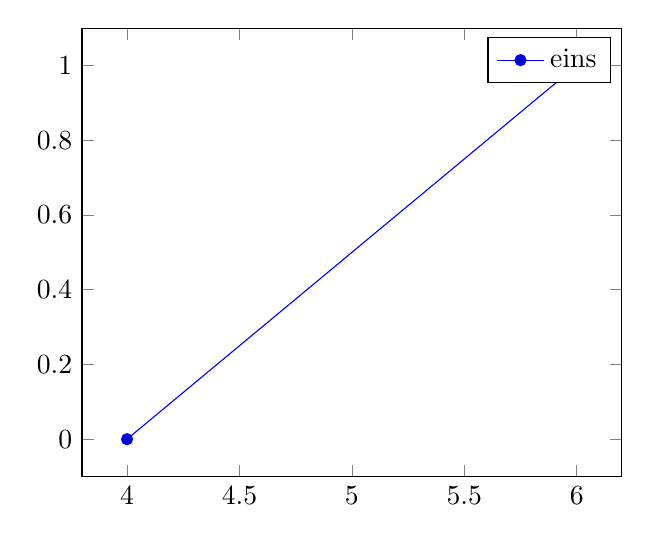
\begin{tikzpicture}
\begin{axis}
\smallplotstest

\addplot plot coordinates {
	(4,0)
	(6,1)
};
\legend{eins\\zwei\\}%
\end{axis}
\end{tikzpicture}

\item MIT aenderung:

\begin{tikzpicture}
\begin{axis}
\smallplotstest

\addplot+[only marks] plot coordinates {
	(4,0)
	(6,1)
};
\legend{eins\\zwei\\}%
\end{axis}
\end{tikzpicture}
\end{enumerate}
}

\testsection{Hide axis test}
\begin{tikzpicture}
	\begin{axis}
		\smallplotstest
	\end{axis}
\end{tikzpicture}
\begin{tikzpicture}
	\begin{axis}[hide axis]
		\smallplotstest
	\end{axis}
\end{tikzpicture}
\vskip 1cm
\noindent
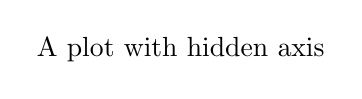
\begin{tikzpicture}
	\begin{axis}[hide axis,title=A plot with hidden axis]
		\smallplotstest
	\end{axis}
\end{tikzpicture}
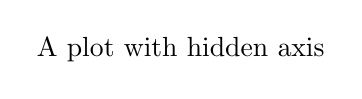
\begin{tikzpicture}
	\begin{axis}[hide axis,title=A plot with hidden axis]
		\smallplotstest
		\legend{A legend\\}
	\end{axis}
\end{tikzpicture}

{
\def\testaxis#1{
	\begin{tikzpicture}
	\begin{axis}[#1,title=A title,xlabel=$x$,ylabel=$y$]
	
	\addplot (\x,\x^2);
	\legend{$x^2$}
	\end{axis}
	\end{tikzpicture}
}
\testsubsection{hide x/y axis}
\testaxis{hide x axis}

\testaxis{hide y axis}

\testaxis{hide x axis,axis y line=center}

\testaxis{hide y axis,axis x line=center}

\testaxis{hide x axis,axis y line=right}

\testaxis{hide y axis,axis x line=bottom}
}

\testsection{disabledatascaling / disablelogfilter}
\testsubsection{disabledatascaling}
\begin{tikzpicture}
\begin{axis}[disabledatascaling]
	\smallplotstest
\end{axis}
\end{tikzpicture}

\testsubsection{disabledatascaling + explicit limits}
\begin{tikzpicture}
\begin{axis}[disabledatascaling, xmin=0, xmax=1, ymin=0, ymax=1]
	\smallplotstest
\end{axis}
\end{tikzpicture}

\testsubsection{disabledatascaling + explicit limits + error bars}
\begin{tikzpicture}
\begin{axis}[disabledatascaling, xmin=-0.5, xmax=1.5, ymin=-0.5, ymax=1.5]
\addplot plot[
	/pgfplots/error bars/.cd,
	y dir=both,y explicit,
	x dir=both,x fixed relative=0.5,
	error mark=diamond*,
]
	coordinates
	{(0,0) +- (0.5,0.1) 
	(0.1,0.1)  +- (0.05,0.2)
	(0.2,0.2) 	+- (0,0.05)
	(0.5,0.5)
	(1,1)};
\end{axis}
\end{tikzpicture}
